\documentclass{report}

\usepackage{url}
\usepackage{indentfirst}
\usepackage{float}

\usepackage{amsmath}
\usepackage[T1]{fontenc}
\usepackage{textcomp} % Required for upquote.
\usepackage{listings} % Include the listings-package
% Ensure quotes in listings are straight.
% Cleaner way to print strings in listings packages so no space symbol.
\lstset{showstringspaces=false, upquote=true} 

% eref puts parenthesis around reference, like "equation (1)"
\def\eref#1{(\ref{#1})}
% Used to generate || || (Norm) symbol for Paikin and Tal
\newcommand{\norm}[1]{\left\lVert#1\right\rVert}


\usepackage{mdframed}
\usepackage[numbers,sort]{natbib}
%\usepackage[english]{babel} % Need for text wrap in table.
\usepackage{array} % Needed for centering in the table
\usepackage[export]{adjustbox} % loads also graphicx
\usepackage{graphicx}

\usepackage{hyperref} % Creates links in the PDF document.
\hypersetup{hidelinks} % Do not include boxes around links

% Defines the table of contents depth and the subsection numbering depth
\setcounter{secnumdepth}{5}
\setcounter{tocdepth}{5}

\title{An Enhanced Jigsaw Puzzle Solver \\[1in]
	   CS297 Final Report}

\author{
  Zayd Hammoudeh \\
  (zayd.hammoudeh@sjsu.edu)
  }


\newcommand{\myparagraph}[1]{\paragraph{#1}\mbox{}\\}

% Skip lines after each paragraph.
\setlength\parskip{\baselineskip}

\begin{document}

\maketitle

\pagenumbering{roman}

\tableofcontents{\protect\newpage}

\addcontentsline{toc}{section}{List of Figures}
\listoffigures
\newpage
 
\pagenumbering{arabic}

\renewcommand\thesection{\arabic{section}}

\section{Introduction}\label{sec:introduction}

Jigsaw puzzles have been around since the 1760s when they were made from wood.  Their name derives from the fact that they were originally carved using jigsaws.   The 1930s saw the introduction of the modern jigsaw puzzle where an image was printed on a cardboard sheet that was cut into a set of interlocking pieces \cite{williams1990, williams2004}.  Although jigsaw puzzles had been solved by children for centuries, it was not until 1964 that the first automated jigsaw puzzle solver was proposed by \cite{freeman1964}, and that solver could only solve 9 piece puzzles.  While an automated jigsaw puzzle solver may seem trivial, it has been shown by \cite{altman1990} and \cite{demaine2007} to be strongly NP-complete when pairwise compatibility between pieces is not a reliable metric for determining adjacency.

A jig swap puzzles are specific type of jigsaw puzzle where  all pieces are equally sized, non-overlapping squares.  Jig swap puzzles are substantially more difficult to solve than standard jigsaw puzzle as one can not consider mechanical compatibility when trying to determine affinity between pieces.  As such, one can only consider the image information on each individual piece when solving the puzzle.  

Solving a jigsaw puzzle simplifies to reconstructing an object from a set of component pieces.  As such, techniques developed for jigsaw puzzles can be generalized to many practical problems.  Examples where jigsaw puzzle solving strategies are applicable include: reassembly of archaeological artifacts \cite{brown2008, koller2006}, forensic analysis of deleted files \cite{garfinkel2010}, image editing \cite{cho2008}, reconstruction of shredded documents \cite{zhu2008}, DNA fragment reassembly \cite{marande2007}, and speech descrambling \cite{zhao2007}.

Unlike traditional jigsaw or jig swap puzzles, the original (i.e. target) image is unknown for most practical applications.  This significantly complicates solving the problem as one must determine the overall structure of the complete solution solely from a bag of individual pieces with unknown relationships.

This project proposes an improved jig swap puzzle solver.  It also studies the fundamental structures within images to determine which images are easy or difficult to solve using current techniques.  This study will help guide future research by focusing on the weaknesses with state of the art approaches. 

\pagebreak
\section{Previous Work}\label{sec:previousWork}

Computational solvers for jigsaw puzzles have been studied since the 1960s when Freeman and Garder proposed an approach that could solve jigsaw puzzles of up-to nine pieces using solely the piece shapes \cite{freeman1964}.  Since then the focus of research has shifted from traditional jigsaw puzzles to jig swap puzzles.  

Cho \textit{et. al.} \citep{cho2010} proposed in 2010 one of the first modern computational jig swap puzzle solvers; their approach relied on a graphical model build around a set of one or more ``anchor piece(s)''; these one or more anchor pieces were fixed in their correct location before the the solver began.  Cho \textit{et. al.} also assumed knowledge regarding the size of the puzzle dimensions.  Future solvers would on Cho \textit{et. al.}'s results while also reducing the amount of information passed to the solver beyond the set of pieces.

A significant contribution of Cho \textit{et. al.} is that they were first to use the LAB  (\underline{L}ightness and the \underline{A}/\underline{B} opponent color dimensions) colorspace to encode image pixels (as opposed to standards such as RGB or CMYK) since LAB normalizes the lightness and color variation across all three dimensions.  Cho \textit{et. al.} proposed a measure for quantifying the pairwise distance between two puzzle pieces that became the basis of most of the future work (see \ref{sec:piecePairwiseAffinity} for more details).  

Pomeranz \textit{et. al.} \cite{pomeranz2011} proposed an iterative, greedy jig swap puzzle solver in 2011.  Their solver did not rely on anchor pieces, and the only information passed to the solver were the pieces and the size of the puzzle.  Pomeranz \textit{et. al.} also generalized and improved on Cho \textit{et. al.} piece pairwise distance measure by proposing a ``predictive distance measure''.  Finally, Pomeranz \textit{et. al.} proposed the concept of ``best buddies'', which are two pieces that are more similar to each other than they are to any other pieces.  Best buddies have served as the basis for both an estimation metric for the quality of a solved image as well as the foundation of some solvers' placers \cite{paikin2015}.

In 2012, Gallagher \cite{gallagher2012} formalizes the different categories of jig swap problems into three primary types.  The following is Gallagher's proposed terminology, and his nomenclature is used throughout this document.

\begin{itemize}

	\item \textbf{Type 1 Puzzle}: The dimension of the puzzle (i.e. the width and height of the original image in number of pixels) is known.  What is more, the orientation of each piece is known, which means that there are exactly four pairwise relationships between any two pieces.  A single anchor piece, with a known, correct, location is required with additional anchor pieces being optional.  This type of puzzle is used by \cite{cho2010, pomeranz2011}.
	
	\item \textbf{Type 2 Puzzle}: This is an extension of a type 1, where the rotation of any piece is unknown.  This change alone increases the number of possible solutions by a factor of $4^n$ (where $n$ is the number of pieces in the puzzles) in comparison to a Type 1 puzzle.  What is more, no piece locations are known in advance; this change eliminates the use of anchor piece(s).  Lastly, the dimensions of the original puzzle can be unknown.
	
	\item \textbf{Type 3 Puzzle}: All puzzle piece locations are known and only the rotation of the puzzle pieces is unknown.  This is the least computationally complex of the three puzzle variants and is generally considered the least interesting.  Type 3 puzzles are not explored as part of this thesis.

\end{itemize}

Sholomon \textit{et. al.} also propose a fourth type (i.e. "Type 4") puzzle whereby each puzzle piece has an image on both sides.  Each puzzle is similar to a 

\pagebreak
\section{Puzzle Piece Pairwise Affinity}\label{sec:piecePairwiseAffinity}

Pairwise affinity quantifies the similarity between the edges of two puzzle pieces.  $D(x_i, s_i, x_j, s_j)$ and $C(x_i, s_i, x_j, s_j)$ represent the distance and compatibility (i.e. similarity) between side $s_i$ of puzzle piece $x_i$ and side $s_j$ of puzzle piece $x_j$.  

\subsection{Cho \textit{et. al.} Pairwise Affinity}\label{sec:choPairwiseAffinity}

As mentioned in section \ref{sec:previousWork}, Cho \textit{et. al.} \cite{cho2010} proposed one of earliest edge-based pairwise affinity measures for two puzzle pieces.  Their approach is shown in Equation~\eref{eq:choPairwise}, which quantifies the distance between the left (``$L$'') side of piece $x_i$ and the right (``$R$'') side of piece $x_j$.  $K$ is the width/height of a puzzle piece in number of pixels\footnote{Cho \textit{et. al.} used 7 for $K$.}.  

\begin{equation} \label{eq:choPairwise}
D(x_i,L,x_j,R) = \sum_{k=1}^{K}\sum_{d=1}^{3}(x_i(k,K,d) - x_j(k,1,d))^2
\end{equation}

Since the LAB colorspace has three dimensions (e.g. lightness and A/B opponent colors), $d$ ranges between $1$ and $3$.  Similarly, $x_i(k,K,d)$ represents the LAB value in dimension $d$ of the pixel in row ``$k$'' of column $K$ in piece $x_i$.

\subsection{Pomeranz \textit{et. al.} Pairwise Affinity}\label{sec:pomeranzPairwiseAffinity}

One of the disadvantages of Cho \textit{et. al.}'s metric is that it simply squares the difference between the piece's pixel dimensions.  It is possible that superior results may be achieved by allowing the solver to modify this exponent term.  Pomeranz \textit{et. al.} in \cite{pomeranz2011} generalize Equation~\eref{eq:choPairwise} using the $L_p$ norm as shown in Equation~\eref{eq:pomeranzPairwise}\footnote{Pomeranz \textit{et. al.} used 28 for $K$.  This has generally become the standard in subsequent papers.}.

\begin{equation} \label{eq:pomeranzPairwise}
D(x_i,L,x_j,R) = \bigg(\sum_{k=1}^{K}\sum_{d=1}^{3}(|x_i(k,K,d) - x_j(k,1,d)|)^p\bigg)^{\frac{q}{p}}
\end{equation}

Hence, for a distance measure equivalent to that of Cho \textit{et. al.}, $p$ and $q$ are set equal to $2$.

An additional down side of the metric proposed by Cho \textit{et. al.} is that it only considers the border pixels.  Hence, if there is some gradient in the original image, two pieces may appear artificially dissimilar using this approach.  To address this issue, Pomeranz \textit{et. al.} proposed predictive compatibility.  Equation~\eref{eq:pomeranzPredCompat} shows the predictive compatibility between the left (``$L$'') side of piece $x_i$ and the right (``$R$'') side of piece $x_j$.  

\begin{equation} \label{eq:pomeranzPredCompat}
\begin{split}
C(x_i,L,x_j,R) = \sum_{k=1}^{K}\sum_{d=1}^{3}\Big[ ([2x_i(k, K, d) - x_i(k, K-1, d)] - x_j(k, 1, d))^p \\ - ([2x_j(k, 1, d) - x_i(k, 2, d)] - x_i(k, K, d))^p\Big]^{\frac{q}{p}}
\end{split}
\end{equation}

Note that in Equation~\eref{eq:pomeranzPredCompat}, the difference between the column of pixels adjacent to the edge is used to account for any gradient effects.

\subsection{Paikin \& Tal Pairwise Affinity}\label{sec:paikinPairwiseAffinity}

Paikin \& Tal in \cite{paikin2015} used Pomeranz \textit{et. al.}'s predictive compatibility as the foundation of their asymmetric distance measure.  Paikin \& Tal's approach is shown in Equation~\eref{eq:paikinAsymDistance}.

\begin{equation} \label{eq:paikinAsymDistance}
D(x_i,L,x_j,R) = \sum_{k=1}^{K}\sum_{d=1}^{3} \norm{[2x_i(k, K, d) - x_i(k, K-1, d)] - x_j(k, 1, d)}
\end{equation}

Note that Paikin \& Tal set $p$ and $q$ equal to 1 as it not only increased the accuracy of the solver but also significantly reduced the computational time.  It is important to note that since this distance is asymmetric, in most cases $D(x_i,L,x_j,R)$ will not equal $D(x_j,R,x_i,L)$.

Pomeranz \textit{et. al.} only considered the relationship between two individual pieces when determining the pairwise compatibility.  In images (or areas of images) with little variation (e.g. an all white image), parts may have artificially high pairwise distances.  To account for this, Paikin \& Tal proposed asymmetric compatibility as shown in Equation~\eref{eq:paikinAsymCompatibility}.

\begin{equation} \label{eq:paikinAsymCompatibility}
C(x_i,L,x_j,R)=1 - \frac{D(x_i,L,x_j,R)}{secondD(x_i,L)}
\end{equation}

\noindent
where $secondD(x_i,L)$ is the second best asymmetric distance between the left side of piece $x_i$ and all other pieces.  By normalizing compatibility with respect to the second best match, it is possible to identify those pairings that have actually have high compatibility while at the same time removing the artificially high compatibilities between pieces from areas of the image with low variation.

\subsubsection{Improved Asymmetric Compatibility}\label{sec:hammoudehPairwiseAffinity}

In an image that was generated from an analog input (e.g. a photograph), it is expected that there will be some degree of natural variation across the image due to variations in brightness, the object in the photo, and the image sensor.  However, in digital images that are generated or manipulated by computers, this variation can be trivially removed.  An example of this would be an image of a solid color or object(s) in front of a white background as shown in figure~\ref{fig:objectWhiteBackground}.

\begin{figure}
\centering
\fbox{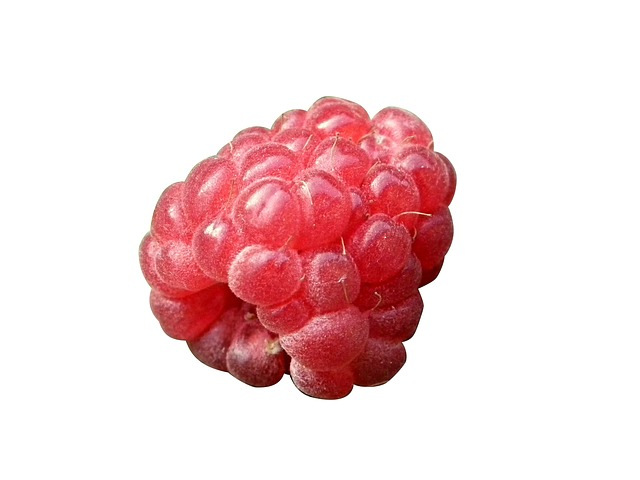
\includegraphics[width=50mm]{./images/raspberry_pixabay.jpg}}
\caption{A Computer Manipulated Image with Poor Asymmetric Compatibility}
\label{fig:objectWhiteBackground}
\end{figure}

The puzzles pieces along the border of the image as well as the pieces in the background have sides that are all white.  This entails that regardless of which of the three metrics are used, the distance between them is zero.  What is more, Paikin \& Tal do not explicitly define how to handle this case for asymmetric compatibility.  Therefore, to better handle computer generated images, this thesis proposes an enhanced definition of asymmetric compatibility as shown in Equation~\eref{eq:hammoudehAsymCompatibility}.  

\begin{equation} \label{eq:hammoudehAsymCompatibility}
C(x_i,L,x_j,R)= \begin{cases} 
	1 - \frac{D(x_i,L,x_j,R)}{secondD(x_i,L)} & secondD(x_i,L) \ne 0
\\
	-\alpha & secondD(x_i,L) = 0
\end{cases} 
\end{equation}

\noindent
where $\alpha$ is a penalty term that denotes that such pairings have low compatibility.


\subsection{Best Buddies}\label{sec:bestBuddies}

As defined by Pomeranz \textit{et. al.}, two pieces, $x_i$ and $x_j$ are best buddies on their respective sides $s_i$ and $s_j$ if they are more compatible (i.e. similar) to each other than they are to each other.  This is more formally described in Equation~\eref{eq:bestBuddyDefinition}.

\begin{equation} \label{eq:bestBuddyDefinition}
\begin{split}
\begin{matrix}
\forall{x_k} \forall{s_k} \in Parts, & C(x_i, s_i, x_j, s_j) \geq C(x_i, s_i, x_k, s_k)
\\
\\
\multicolumn{2}{c}{\textnormal{and}}
\\
\\
\forall{x_k} \forall{s_k} \in Parts, & C(x_j, s_j, x_i, s_i) \geq C(x_j, s_j, x_k, s_k)
\end{matrix}
\end{split}
\end{equation}

The definition of best buddies applies regardless of whether the compatibility definition of Pomeranz \textit{et. al.} or Paikin \& Tal is used.

\subsubsection{An Improved Best Buddies Definition}\label{sec:bestBuddiesLimitations}

In photographs, it is generally unlikely that there will be a significant number of cases where a piece has multiple best buddies on the same side.  However, in computer generated or computer manipulated images where there may be solid colors or backgrounds, that is far more common.  To address issues of this type, this thesis proposes a modified definition of best buddies as shown in Equation~\eref{eq:hammoudehBestBuddyDefinition}.

\begin{equation} \label{eq:hammoudehBestBuddyDefinition}
\begin{split}
\begin{matrix}
\forall{x_k} \forall{s_k} \in Parts, & C(x_i, s_i, x_j, s_j) > C(x_i, s_i, x_k, s_k)
\\
\\
\multicolumn{2}{c}{\textnormal{and}}
\\
\\
\forall{x_k} \forall{s_k} \in Parts, & C(x_j, s_j, x_i, s_i) > C(x_j, s_j, x_k, s_k)
\end{matrix}
\end{split}
\end{equation}

Rather than relying on best buddies being ``greater than or equal'' to all other pieces, the modified requirement is that pairings must be strictly greater than.  Hence, best buddy pairings are exclusive with cliques of size greater than two being explicitly disallowed.

\pagebreak
\bibliographystyle{ieeetr}
\bibliography{cs297_final_report_biblio}

\end{document}
